\chapter{Frontend}

Možnosti tvorby webových aplikací se posledních několik let rapidně zvětšují. Prohlížeče implementují stále nové technologie, které royšiřují možnosti.

\section{Možnosti programování frontendu}

Programátor webového frontendu si dnes může vybírat z několika paradigmat tvorby webové stránky. Standardem je dnes programovací jazyk Javascript. Spíše historicky bylo výhodné místo Javascriptu používat pro frontendový vývoj různé pluginy. Nejznámější je Adobe Flash, nebo Microsoft Silverlight. Programovat pro tyto pluginy mělo velké výhody. Například snadné přehrávání videa, zobrazení stránky v celoobrazovkovém režimu, nebo přístup k uživatelově webkameře. V době, kdy byla Javascriptová API velmi chudá a rozdílně implementovaná mezi prohlížeči, nabízel Flash zejména tvůrcům webových her konzistenci mezi všemi platformami.

Velkou nevýhodou těchto pluginů byla jejich proprietálnost. Ostatní firmy se bály pustit cizí plugin do svých výrobků. Zlomový moment pro ústup Flashe ze slávy bylo uvedení telefonu iPhone, který podporu pro Flash nenabízel. Softwareoví giganti Microsoft, Apple a Google začali místo proprietálních řešení tlačit otevřenou specifikaci, která se později nazvala HTML5. HTML5 je zastřešující termín pro spoustu technologií, které snaží webová API specifikovat a vytvářet nové.

\section{JavaScriptové frameworky}

Druhým hnacím motorem moderního Javascriptu jsou frameworky. Ještě před několika lety byla práce na interaktivních webech velmi náročná. Prohlížeče se zásadně lišily v implementaci práce s eventy a DOMem. Nové frameworky do jisté míry odstínily programátora od odlišných implementací Javascriptu v prohlížečích.

\subsection{jQuery}
Nejpopulárnějším frameworkem současnosti je jQuery. Ten nabízí jednoduché rozhraní a pro velkou většinu menších webových aplikací je zcela dostačující. Čím je ale aplikace větší, tím začíná být její vývoj s pomocí jQuery náročnější. Zkusme ukázat, jak by v jQuery vypadalo přidání CSS třídy red oknu s id okno:

\begin{lstlisting}
  $("#okno").addClass("red");
\end{lstlisting}

Kód má několik problémů. Pokud neexistuje žádné okno s id okno, jQuery nevrátí žádnou chybu. Stačí malý překlep a chyba v kódu se hledá dost obtížně. jQuery nenabízí žádnou funkci typu vratObjektPodleId. Pokud by tyto funkce nabízel, velikost jeho kódu by se zvětšila. Pokud chce programátor použít knihovnu jQuery, musí si ji uživatel stránky celou stáhnout. Verze XX má XX bajtů.

\subsection{Google Closure}
Jiný přístup k vývoji frontendových aplikací přináší Google. Pro svou první webovou aplikaci Gmail vyvinul sadu nástrojů, kterou později vydal jako open source pod názvem Google Closure. Kromě Gmailu ji Google využívá v Google Vyhledávání, Google Mapách, nebo Google Dokumentech. Skládá se ze tří částí - Closure Compiler, Closure Library a Closure Templates. Closure Library je obsáhlá knihovna funkcí pro práci s DOMem, Eventy, matematickými výpočty a spoustou dalších věcí, které webový programátor může využít.

Closure Compiler je inteligentní minifikátor Javascriptového kódu. Odstraňuje funkce, které nejsou volány, přejmenovává všechny názvy funkcí a proměnných na co nejkratší řetězce a v ADVANCED módu se snaží i o pokročilejší optimalizace kódu (například kód funkcí, které jsou volány pouze jednou, je vlože inline). Nejlepích výsledků dosahuje s použitím speciálních anotací, které například vynucují typ proměnné a jsou schopny udělat z Javascriptu typovaný jazyk. Closure Compiler tyto anotace vyhodnocuje a při chybném přiřazení hodnoty vrátí chybu. To umožňuje tvořit více bezpečný javascriptová kód.

Třetí částí Google Closure jsou Closure Templates, šablonovací systém pro Javascript a Javu. Pomocí Closure Templates se snadno vytváří zanořené HTML šablony. Všechny uživatelské vstupy jsou escapované což zabraňuje sniffing útokům.

Částí Templates a Compiler jdou použít odděleně v jakémkoliv Javascriptovém projektu. Používat Closure Library be Compileru nedává příliš smysl, uživatel by při návštěvě webu musel stahovat ohromné množství zbytečných dat.

Tato práce na frontendu používá všechny části knihovny Google Closure. Díky tomu si uživatel při první návštěvě webu musí stáhnout pouze jediný soubor, který má pouze XX Kb.

\section{Stylování uživatelského rozhraní a CSS}

Specifikace HTML5 rozšiřuje i možnosti vizualizace pomocí CSS stylů. Nejviditelnějšími novinkami je podpora kulatých rohů, stínování, nebo barevných přechodů. Webový programátor nyní může ke stránce načíst i vlastní font. Všechny tyto možnosti velmi rozšířily možnosti webovým grafikům.

Dalším trendem, který v CSS světě probíhá, je používání CSS preprocesorů. 


\section{Uživatelské rozhraní}

\begin{figure}[h]
  \centering
  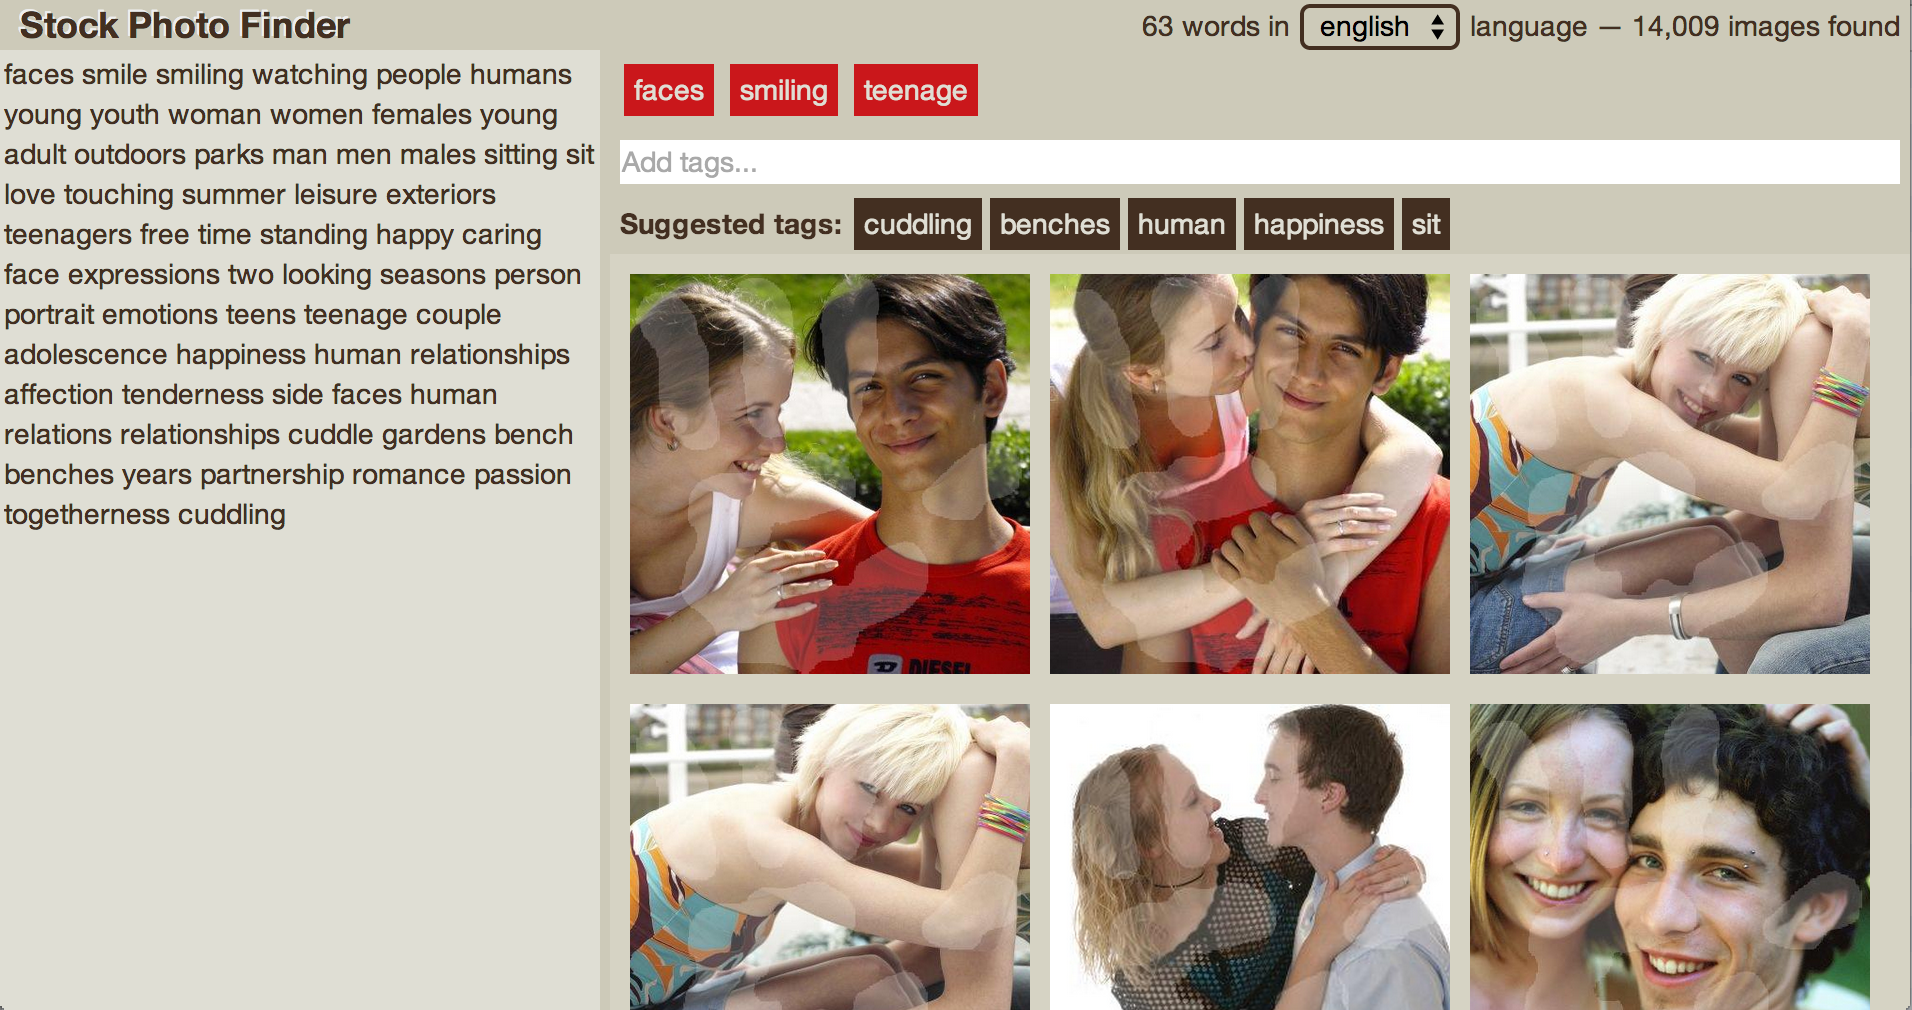
\includegraphics[width=150mm]{ui1.eps}
  \caption{Ukázka čtverců algoritmu Geohash v jednotkovém čtverci.}
  \label{fig:ui1}
\end{figure}




